\chapterWithSubtitle{Non-Regularity and Fooling Sets}{February 16, 2021}

\section{Proving Non-Regularity: Methods}
\begin{itemize}
    \item \textbf{Pumping Lemma}: (Not covered in CS 374)
    \item \textbf{Closure}: Use existing non-regular languages and regular languages to prove that some new language is non-regular. to prove that some new  is non-regular.
    \item \textbf{Fooling Sets}: Method of distinguishing suffixes. To prove that $L$ is non-regular, find an infinite fooling set.
\end{itemize}

\subsection{Closure Properties}
\begin{itemize}
    \item Suppose $L = L_1 \cap L_2$, and we know that $L_2$ is regular.
    \item Because regular languages are closed under intersection:
    \begin{itemize}
        \item If $L_1$ is regular, then $L$ is regular.
        \item If $L_1$ is not regular, then $L$ is not necessarily regular.
    \end{itemize}
\end{itemize}

\subsection{Regular Languages, Finite Automata}
\begin{itemize}
    \item \textit{Theorem}: Languages accepted by DFAs, NFAs, and regular expressions are the same.
    \item \textit{Theorem}: $L = \{ 0^n 1^n \mid n \geq 0 \}$ is not regular:
    \begin{itemize}
        \item \textit{Intuition}: Any program to recognize $L$ seems to require counting the number of zeros in input which cannot be done with fixed memory.
        \item Suppose $L$ is regular. Then there is a DFA $M$ such that $L(M) = L$. $\lvert Q_M \rvert = \left \lceil{n^2}\right \rceil$.
        \item $n$ is unbounded, so $\left \lceil{n^2}\right \rceil$ is also unbounded.
    \end{itemize}
\end{itemize}

\subsection{Comparing States}
\begin{itemize}
    \item DFA $M = (Q, \sum, \delta, s, A)$
    \item Two states $p,q \in Q$ are \textbf{equivalent} if for all strings $w \in \sum^{\ast}$, we have that $\delta^{\ast}(p, w) \in A \iff \delta^{\ast}(q, w) \in A$. One can merge any two states that are equivalent into a single state.
    \item Two states $p,q \in Q$ are \textbf{distinguishable} if there exists a string $w \in \sum^{\ast}$, such that $\delta^{\ast}(p, w) \in A \text{ and } \delta^{\ast}(q, w) \notin A$, or $w \in \sum^{\ast}$, such that $\delta^{\ast}(p, w) \notin A \text{ and } \delta^{\ast}(q, w) \in A$.
    \item \textit{Idea}: Every string $w \in \sum^{\ast}$ defines a state $\nabla w = \delta^{\ast}(s,w)$.
    \item \textit{Definition}: Two strings $u, w \in \sum^{\ast}$ are \textbf{distinguishable} for $M$ or $L(M)$ if $\nabla u$ and $\nabla w$ are distinguishable.
    \item \textit{Definition (Direct restatement)}: Two prefixes $u, w \in \sum^{\ast}$ are \textbf{distinguishable} for a language $L$ if there exists a string $x$, such that $ux \in L$ and $wx \notin L$ (or $ux \notin L$ and $wx \in L$).
\end{itemize}

\subsection{Fooling Set}
\begin{itemize}
    \item For a language $L$ over $\sum$, a set of strings $F$ (could be infinite) is a \textbf{fooling set} or \textbf{distinguishing set} for $L$ if every two distinct strings $x, y \in F$ are distinguishable.
    \item Suppose $F$ is a fooling set for $L$. If $F$ is finite, then there is no DFA $M$ that accepts $L$ with less than $\left|{F}\right|$ states.
    \item If $L$ has an infinite fooling set $F$, then $L$ is not regular.
\end{itemize}

\section{Exponential Gap Between NFA and DFA Size}
\begin{itemize}
    \item $L_k = \{ w \in \{ 0, 1 \}^{\ast} \mid \text{$w$ has a 1 $k$ positions from the end} \}$
    \item Recall that $L_k$ is accepted by a NFA $N$ with $k+1$ states.
    \item \textit{Theorem}: Every DFA that accepts $L_k$ has atleast $2^k$ states.
    \item \textit{Claim}: $F = \{ w \in \{ 0, 1 \}^{\ast}: \left|w\right| = k \}$ is a fooling set of size $2^k$ for $L_k$.
    \item[] 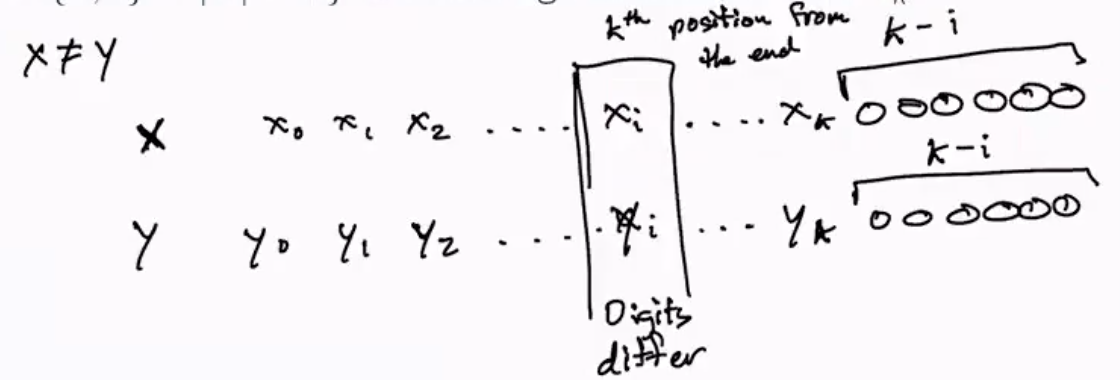
\includegraphics[width=\textwidth]{lecture7/images/fooling-set-2^k.png}
\end{itemize}

\section{Myhill-Nerode Theorem}
\begin{itemize}
    \item \textbf{Myhill-Nerode Theorem}: A regular language $L$ has a unique (up to naming) minimal automata and it can be comuted efficiently once any DFA is given for $L$.
\end{itemize}
